\chapter{Introduction}
\label{Introduction}

\section{Motivation}

\overridetextsize
Deep neural networks (DNNs) have succeeded on numerous tasks, from image and
speech recognition \cite{russakovsky_imagenet_2015,amodei_deep_2015} to
self-driving cars \cite{bojarski_end_2016} and beating the world champion at
the game of Go \cite{silver_mastering_2016}. However, despite achieving
state-of-the-art performance in various domains, deep neural networks are
vulnerable to adversarial examples \cite{szegedy_intriguing_2014}, \emph{i.e.},
inputs containing a carefully crafted perturbation that causes an image
classification model to make the wrong predictions as seen in figure
\ref{fig:adversarial_examples}.

\begin{figure}[!htb]
    \centering
    \subfloat[\centering]{{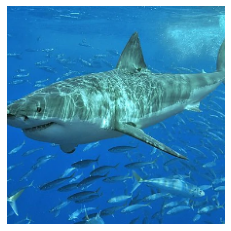
\includegraphics[width=.33\linewidth]{figures/intro/normal.png}}} %
    \subfloat[\centering]{{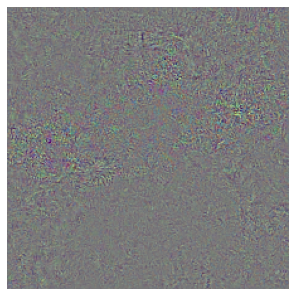
\includegraphics[width=.33\linewidth]{figures/intro/ae_diff.png}}} %
    \subfloat[\centering]{{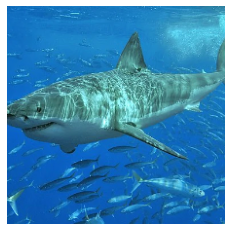
\includegraphics[width=.33\linewidth]{figures/intro/ae.png}}} %
    \caption{Normal image (A), adversarial perturbation (B), adversarial
        example (C). The model accurately classifies the normal image as a
        "white shark" while misclassifying the adversarial example as a "prairie
        chicken."}
    \label{fig:adversarial_examples}
\end{figure}

Researchers demonstrated this phenomenon to be observable not only in computer
vision, but also in speech recognition \cite{carlini_audio_2018} by showing that
a perturbed audio waveform could make a speech-to-text model drastically change
the transcription, as seen in figure \ref{fig:carlini_audio}.
\begin{figure}[!htb]
    \centering
    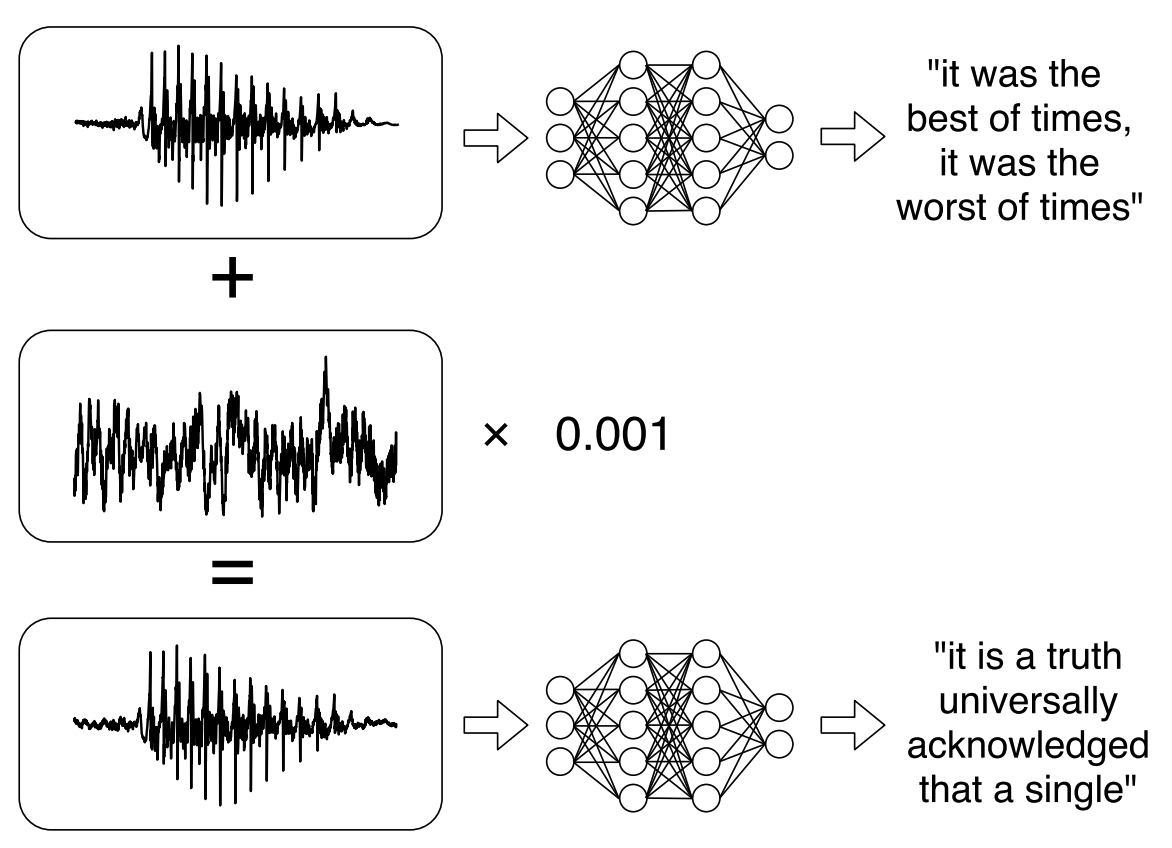
\includegraphics[width=.6\linewidth]{Figures/intro/carlini_noise.png}
    \caption{ Unnoticeable audio waveform added to an audio recording changes
        the transcription by the model drastically \cite{carlini_audio_2018}.}
    \label{fig:carlini_audio}
\end{figure}



One surprising aspect of these adversarial examples is that, as seen in figure
\ref{fig:adversarial_examples} or figure \ref{fig:noise}, the perturbation
needed to fool a model into misclassification can be so small that it is
unnoticeable to a human observer. So small that it was even demonstrated in a
recent study that modifying a single pixel from the input vector can be enough
to fool a neural network in certain circumstances \cite{su_one_2019}, as shown in figure
\ref{fig:su_one_pixel}.

\begin{figure}[!htb]
    \centering
    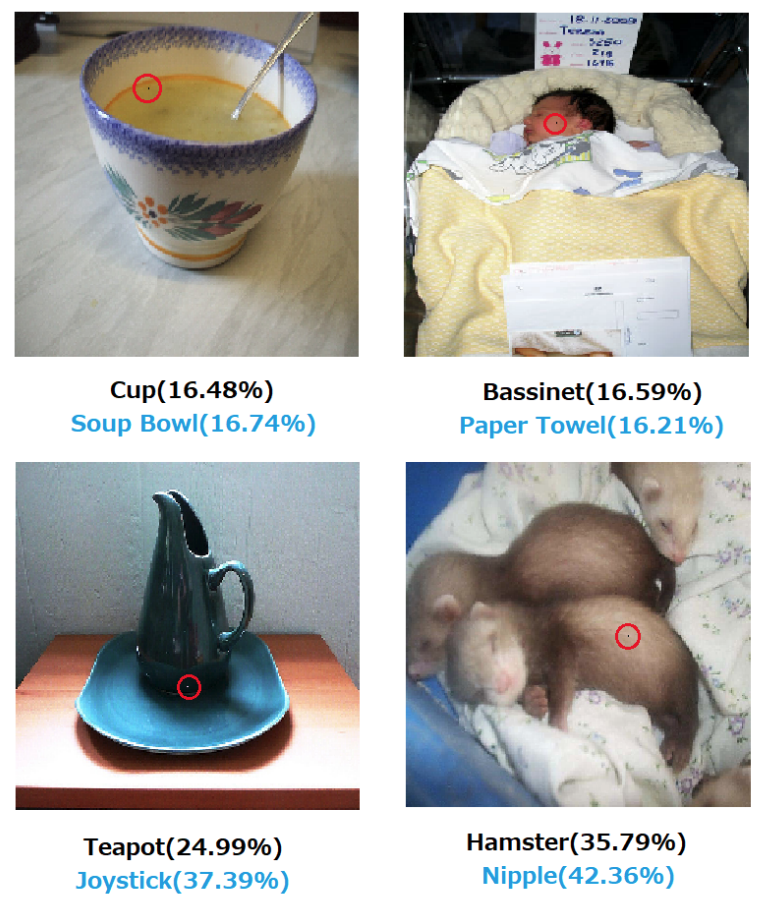
\includegraphics[width=.6\linewidth]{Figures/intro/su_one_pixel.png}
    \caption{ One-pixel attack \cite{su_one_2019}. Modified pixels are
        circled in red. Original predictions in black and predictions with
        modified pixels in blue.}
    \label{fig:su_one_pixel}
\end{figure}

\begin{figure}[!htb]
    \subfloat[]{%
        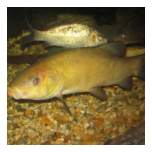
\includegraphics[clip,width=.33\linewidth]{Figures/fig2/Fig2a.png}%
    } \subfloat[]{%
        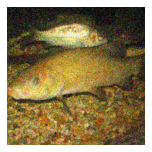
\includegraphics[clip,width=.33\linewidth]{Figures/fig2/Fig2b.png}%
    } \subfloat[]{%
        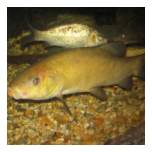
\includegraphics[clip,width=.33\linewidth]{Figures/fig2/Fig2c.png}%
    }

    \caption{ Normal image (A), noisy image (B), adversarial example (C). The
        model accurately predicts both the normal image and noisy image but
        misclassifies the adversarial example, despite the adversarial
        perturbation being $\approx{20}$ times smaller than the random
        perturbation in that case. }
    \label{fig:noise}
\end{figure}

On the other hand, with the constant improvement of neural network architectures
\cite{he_deep_2015,vaswani_attention_2017,huang_densely_2018} and regularization
techniques such as dropout \cite{srivastava_dropout_2014}, neural networks have
become more and more robust against randomly perturbed inputs
\cite{hendrycks_benchmarking_2019}. Thus, as long as the random perturbations
are not too significant, \emph{e.g.}, rotation of the image, compression
deterioration (\emph{e.g.}, JPEG), brightness or contrast shift, the neural
network will still accurately predict the images.

This divergence of robustness displayed by neural networks when facing random
and adversarial perturbations motivated me to experiment with the robustness of
adversarial examples themselves by intentionally adding a random perturbation on
these modified samples.

\clearpage
\section{Main Contribution}
I propose a novel method for detecting adversarial examples based on
intentionally introducing Gaussian noise on the input with varying intensity.
Then, two scores are computed that evaluate the difference of prediction by the
model before applying noise and after, at varying intensity. The advantage of
this method is that the detection efficacy does not rely on prior knowledge
about the attack used and thus can be applied over a wide range of attacks and
at varying adversarial perturbation budgets.

Furthermore, contrary to state-of-the-art defense or detection approaches, my
method is computationally low demanding because no training or optimization of
the model parameters is required.

Lastly, this method can be combined with other detection methods to increase the
overall application's performance. The method I propose emerged after studying
the effects of applying additive Gaussian noise to normal images and adversarial
examples and observing a disparity that, to the best of my knowledge and at the
time of this work, has not been discussed in prior work.

\section{Thesis Structure}
The material described in chapter \ref{RelatedWork} first provides a brief
explanation and general knowledge about neural networks and the different parts
they contain. Then it includes a description of adversarial examples, the
dangers they represent, and the background knowledge needed to generate them,
using different methods emerging from the research community.

Chapter \ref{Experiments} introduces the experiments I conducted and some of the
results that motivated me to pursue and propose the methodology I later present
and describe in chapter \ref{Methodology} which includes the detection
performances.
